\hypertarget{sh__flush_8c}{
\section{sh\_\-flush.c File Reference}
\label{sh__flush_8c}\index{sh_flush.c@{sh\_\-flush.c}}
}


\subsection{Detailed Description}
\begin{Desc}
\item[For internal use only.]
This file contains the implementation of the \hyperlink{dbprim_8h_a178}{sh\_\-flush()} function, used to release all entries in a sparse matrix linked list.\end{Desc}


Definition in file \hyperlink{sh__flush_8c-source}{sh\_\-flush.c}.

{\tt \#include \char`\"{}dbprim.h\char`\"{}}\par
{\tt \#include \char`\"{}dbprim\_\-int.h\char`\"{}}\par


Include dependency graph for sh\_\-flush.c:\begin{figure}[H]
\begin{center}
\leavevmode
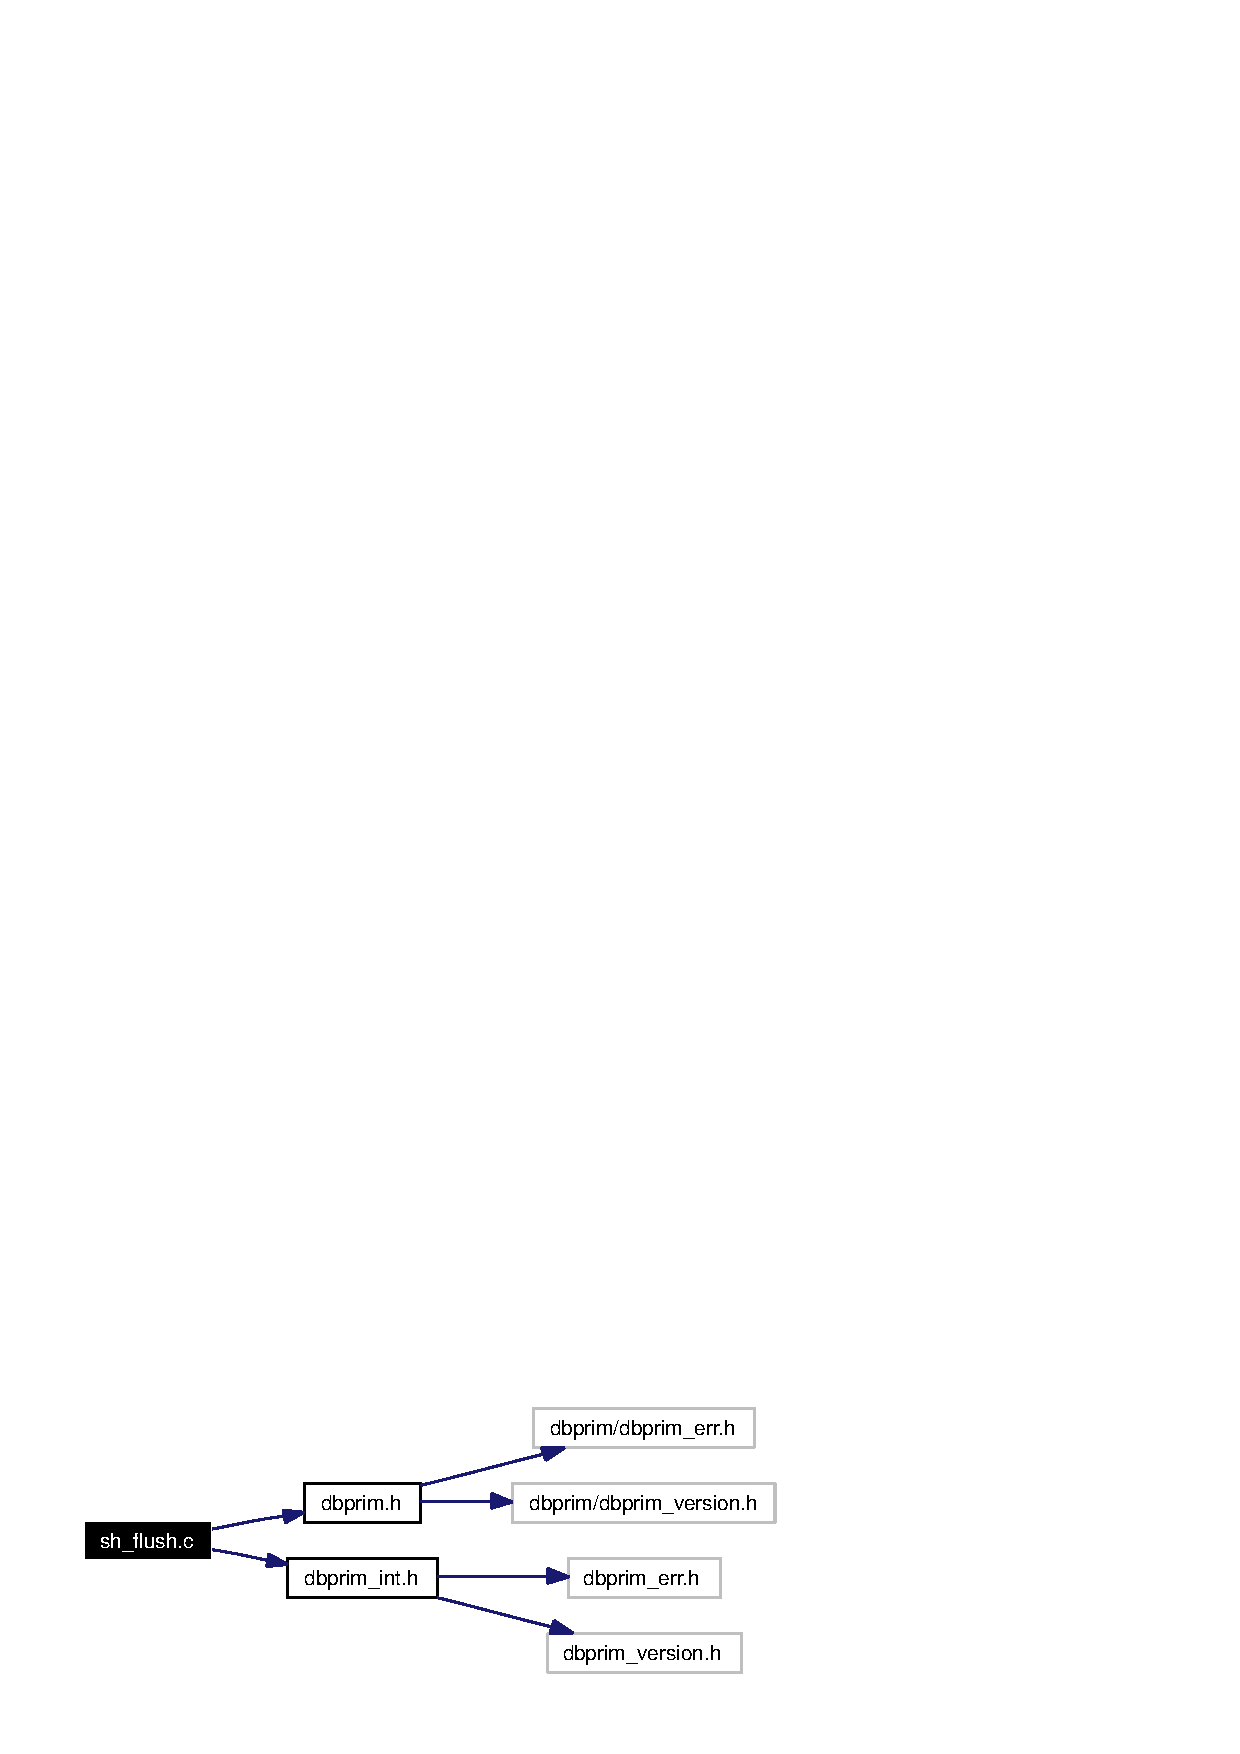
\includegraphics[width=188pt]{sh__flush_8c__incl}
\end{center}
\end{figure}
\subsection*{Data Structures}
\begin{CompactItemize}
\item 
struct \hyperlink{struct__sh__flush__s}{\_\-sh\_\-flush\_\-s}
\begin{CompactList}\small\item\em Sparse matrix flush function shim structure. \item\end{CompactList}\end{CompactItemize}
\subsection*{Functions}
\begin{CompactItemize}
\item 
static unsigned long \hyperlink{group__dbprim__smat_ga28}{\_\-sh\_\-flush\_\-iter} (\hyperlink{struct__link__head__s}{link\_\-head\_\-t} $\ast$head, \hyperlink{struct__link__elem__s}{link\_\-elem\_\-t} $\ast$elem, void $\ast$extra)
\begin{CompactList}\small\item\em Sparse matrix linked list flush callback. \item\end{CompactList}\item 
unsigned long \hyperlink{sh__flush_8c_a1}{sh\_\-flush} (\hyperlink{struct__smat__head__s}{smat\_\-head\_\-t} $\ast$head, \hyperlink{group__dbprim__smat_ga4}{smat\_\-iter\_\-t} flush\_\-func, void $\ast$extra)
\begin{CompactList}\small\item\em Flush a row or column of a sparse matrix. \item\end{CompactList}\end{CompactItemize}


\subsection{Function Documentation}
\hypertarget{sh__flush_8c_a1}{
\index{sh_flush.c@{sh\_\-flush.c}!sh_flush@{sh\_\-flush}}
\index{sh_flush@{sh\_\-flush}!sh_flush.c@{sh\_\-flush.c}}
\subsubsection[sh\_\-flush]{\setlength{\rightskip}{0pt plus 5cm}unsigned long sh\_\-flush (\hyperlink{struct__smat__head__s}{smat\_\-head\_\-t} $\ast$ {\em head}, \hyperlink{group__dbprim__smat_ga4}{smat\_\-iter\_\-t} {\em flush\_\-func}, void $\ast$ {\em extra})}}
\label{sh__flush_8c_a1}


ingroup dbprim\_\-smat

This function flushes a sparse matrix row or column--that is, it removes each element from that row or column. If a {\tt flush\_\-func} is specified, it will be called on the entry after it has been removed from the row or column, and may safely call {\tt free()}.

\begin{Desc}
\item[Parameters:]
\begin{description}
\item[\mbox{$\leftarrow$} {\em head}]A pointer to a \hyperlink{group__dbprim__smat_ga1}{smat\_\-head\_\-t}. \item[\mbox{$\leftarrow$} {\em flush\_\-func}]A pointer to a callback function used to perform user-specifed actions on an entry after removing it from the row or column. May be {\tt NULL}. See the documentation for \hyperlink{group__dbprim__smat_ga4}{smat\_\-iter\_\-t} for more information. \item[\mbox{$\leftarrow$} {\em extra}]A {\tt void} pointer that will be passed to {\tt flush\_\-func}.\end{description}
\end{Desc}
\begin{Desc}
\item[Return values:]
\begin{description}
\item[{\em DB\_\-ERR\_\-BADARGS}]An argument was invalid.\end{description}
\end{Desc}


Definition at line 90 of file sh\_\-flush.c.

References \_\-sh\_\-flush\_\-iter(), ll\_\-flush(), \_\-sh\_\-flush\_\-s::sf\_\-elem, \_\-sh\_\-flush\_\-s::sf\_\-extra, \_\-sh\_\-flush\_\-s::sf\_\-flush, \_\-sh\_\-flush\_\-s::sf\_\-table, \_\-smat\_\-head\_\-s::sh\_\-elem, \_\-smat\_\-head\_\-s::sh\_\-head, \_\-smat\_\-head\_\-s::sh\_\-table, and sh\_\-verify.

Here is the call graph for this function:\begin{figure}[H]
\begin{center}
\leavevmode
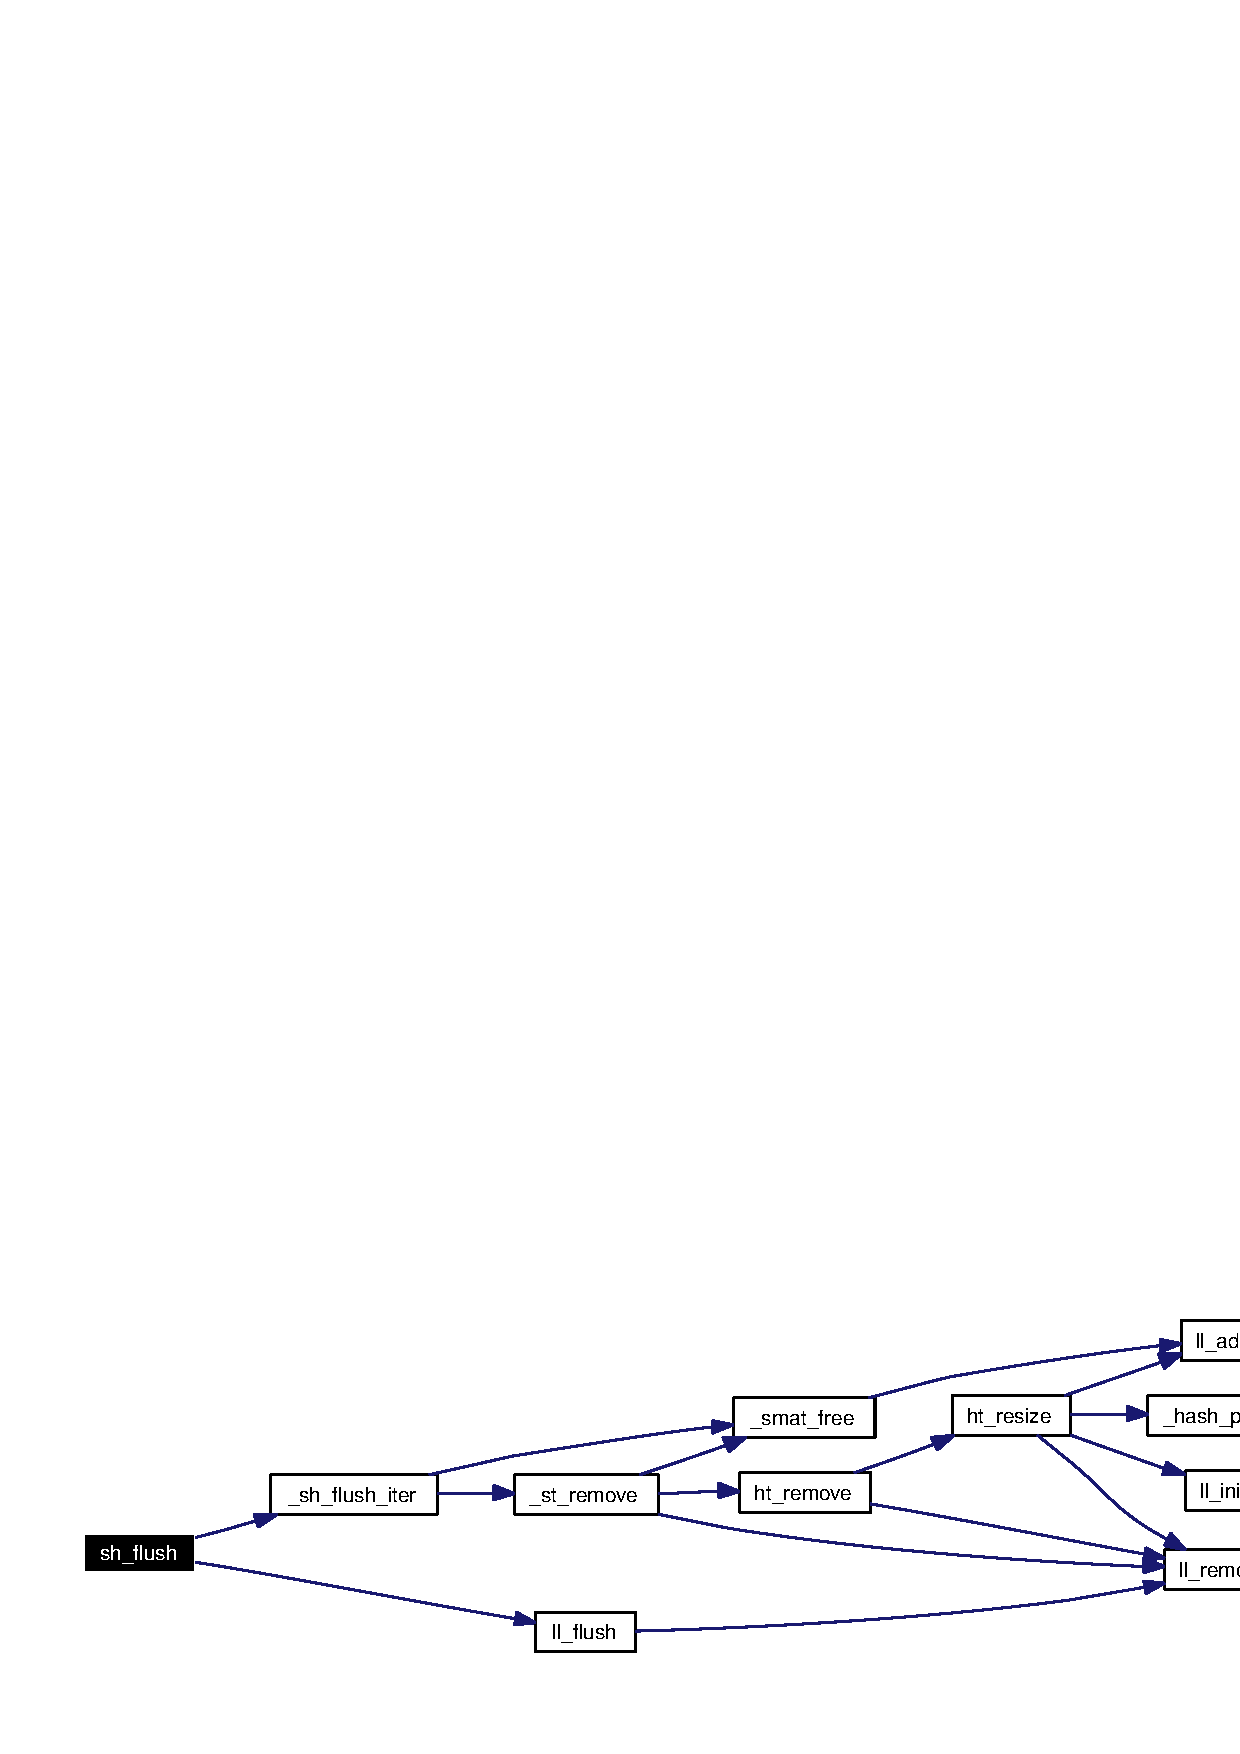
\includegraphics[width=315pt]{sh__flush_8c_a1_cgraph}
\end{center}
\end{figure}
